\documentclass[12pt]{article}

\usepackage{preamble}


\begin{document}
    % Title Page
    \begin{titlepage}
        \center
        \vspace*{1cm}
        \textsc{\LARGE University of Moratuwa}\\[.3cm]
        \textsc{\large ELECTRONIC AND TELECOMMUNICATION ENGINEERING}\\[.3cm]
        \textsc{\large EN3030 : Circuits And System Design}\\[1cm]
        \HRule \\[0.4cm]
        { \LARGE \scshape InFOS: RV32i RISC-V Processor  }\\[0.25cm]
        \HRule \\[2cm]
        
\includegraphics[width=0.5\textwidth]{mora}\\[1.5cm]    % University logo
        {\mdseries Group 12: INFOS}
        \begin{center}
            \begin{tabular}{l l}
                Tharindu O.K.D.       & 190622R \\
                Sanjith. S            & 190562G \\
                Kajhanan K.           & 190286M \\
                Yasarantha D. D. K. B & 190719V \\
                Wansooriya W.H.O.     & 190664V \\
            \end{tabular}
        \end{center}
        {\large \today}\\[.2cm]
        \vfill
        \HRule
        \flushleft {The report is submitted as a partial fulfillment of the module EN3030.}
    \end{titlepage}

    % Table of Contents
    \tableofcontents
    \vspace*{.5cm}
    \listoffigures
    \vspace*{.5cm}
    \listoftables
    \vfill
    \begin{abstract}
        This report presents the design and implementation of a single-cycle Reduced Instruction Set Computer (RISC-V) processor, based on the RV32I instruction set architecture.
        The processor is implemented using Verilog Hardware Description Language and simulated using Verilator together with the GTKWave toolbox.
        The processor includes the basic RISC-V instruction set, including arithmetic, logical, and control flow instructions, and is capable of executing these instructions in a single clock cycle.
        The latter part of the work focuses on a cache controller design for a direct mapped cache bonded with a fully associative victim cache.
    \end{abstract}

    \flushleft{\HRule\\The Executable code can be found \href{https://github.com/University-Academics/INFOS.git}{here}}
    \newpage


    \section{Instruction Set Architecture}
    Based on the requirements of the design it is decided to give support for all 37 instructions of the RV32i instruction set.
    At earlier stages, the instruction encodings are analyzed thoroughly and the results together with instructions are as follows.
    \begin{figure}[h]
        \label{fig:isa}
        \begin{center}
            \rotatebox[origin=c]{90}{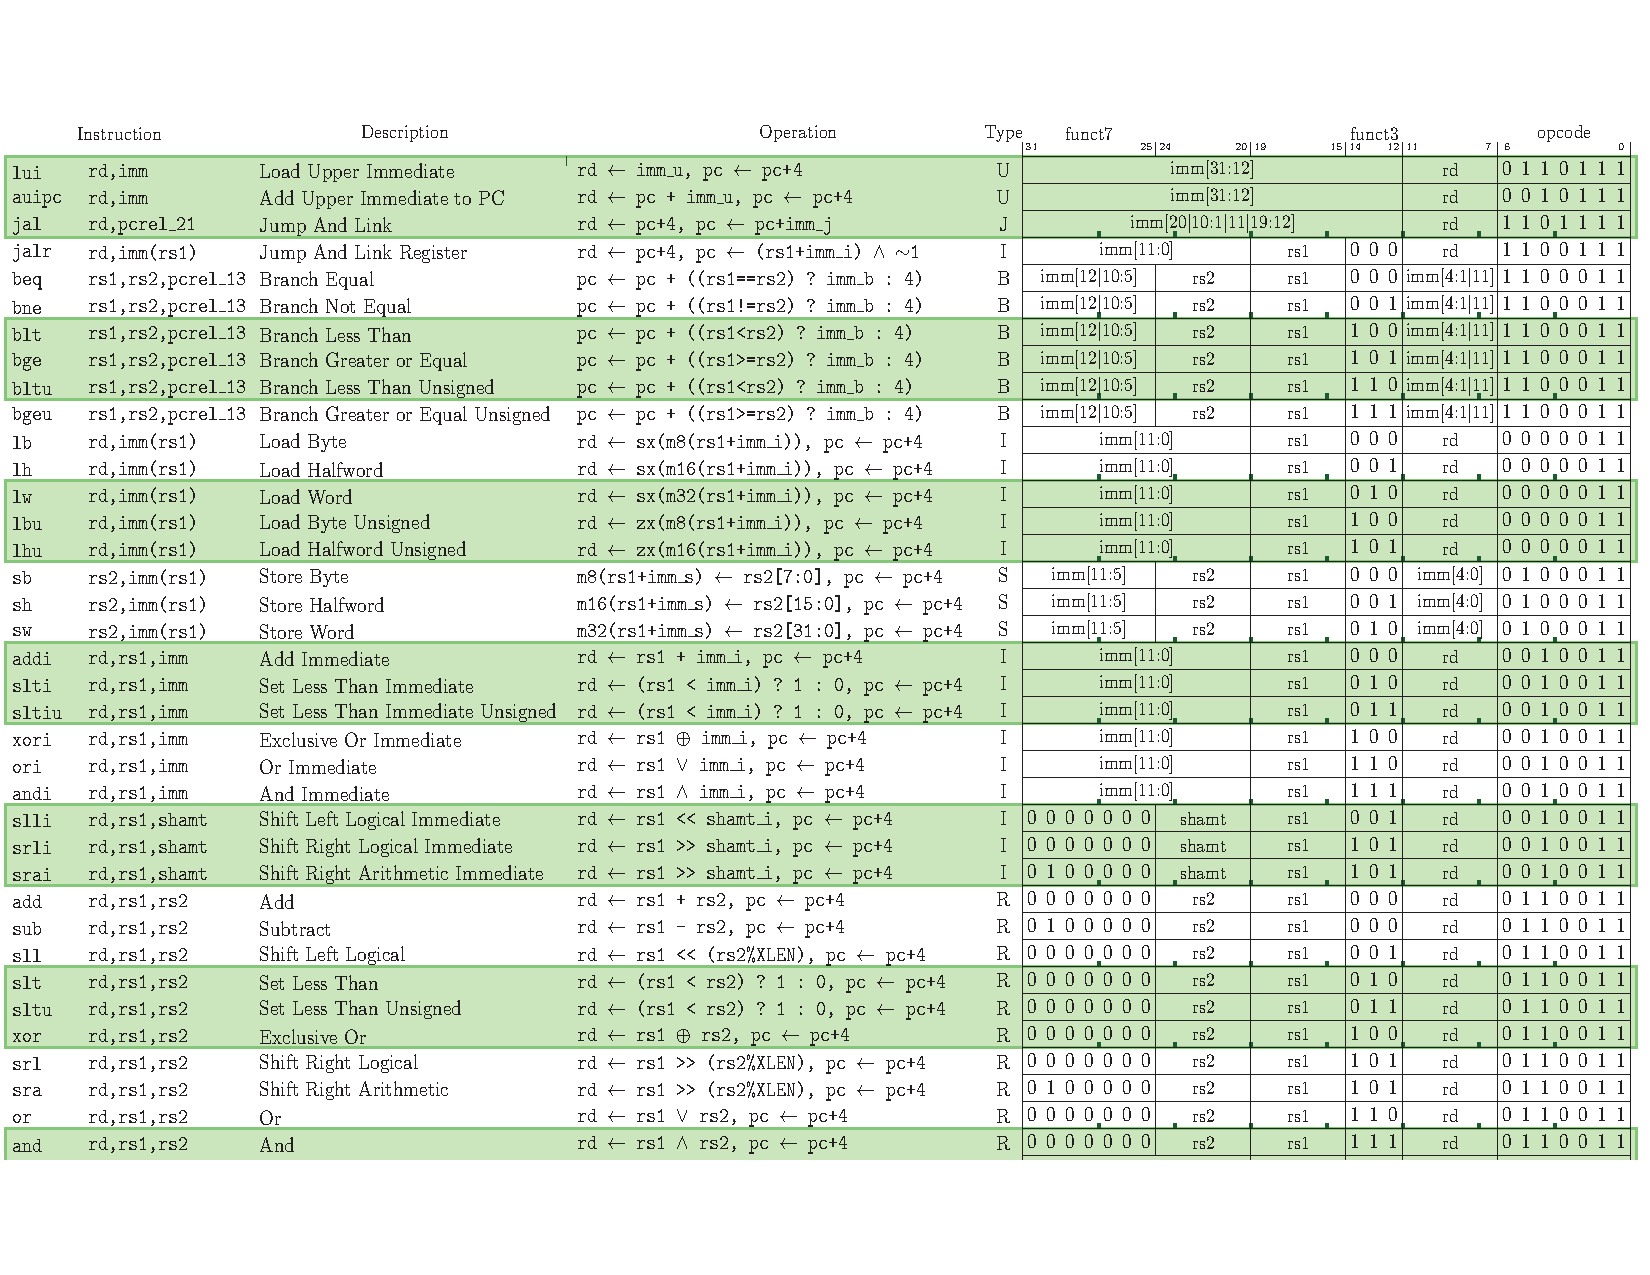
\includegraphics[width=1.22\textwidth,draft = false]{isa}}
        \end{center}
        \comment{RV321-Instruction Set}
    \end{figure}
    \newpage
    \section{Micro Architecture}
    \subsection{Overview}
    \begin{figure}[ht]
        \label{fig:pro}
        \begin{center}
            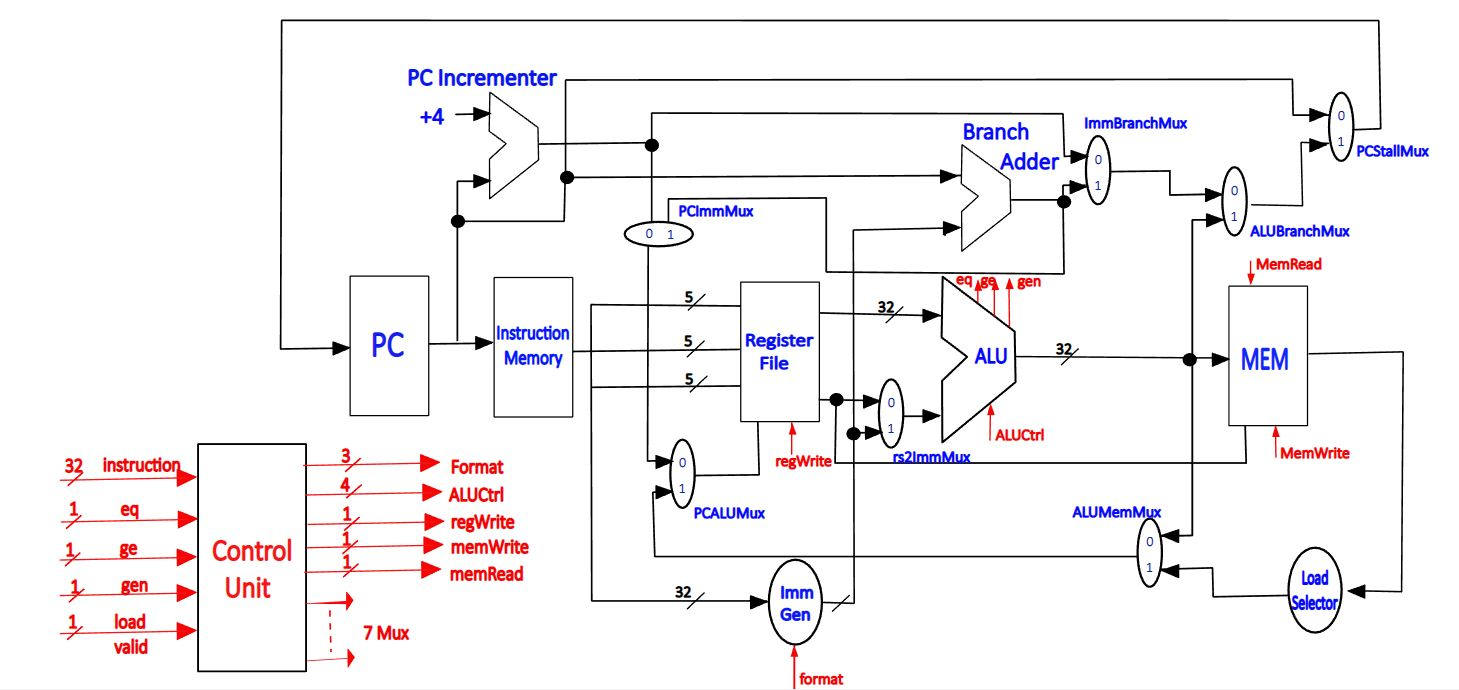
\includegraphics[width=.95\textwidth]{micro}
        \end{center}
        \caption{Micro Architecture Together with Data Paths}
    \end{figure}

    The processor design is completely based on a 32-bit architecture meaning that all the data paths are 32-bit in size.
    The main constituents include a Program Counter, an Instruction Memory, a Register File, a 32-bit ALU, and an Immediate Generator.
    Refer to the next section for more details about these blocks.
    \par
    The branching addresses, on occurrence, when branching instructions are executed, are calculated by a separate adder (Branching Adder indicated in the above figure).
    A separate adder is used to add 4 to the program counter, to find the address of the instruction that is sequentially next to the current instruction.
    For lui, jal, jalr, and auipc instructions, a new Mux is inserted before RegisterFile (PCAluMux) so that the return address can be stored in the rd register.
    \subsection{Register Files}
    Our single-cycle processor architecture demands the register read access through combinational logic and write access at the clock risign edge.
    Totally a 32 different 32-bit registers are implemented.
    Among them x0 register is hard-wired to zero register.
    \subsection{Immediate Generator}
    The immediate generator extracts the corresponding immediate bits from the given instruction according to the type and sign-extends in to a 32-bit number.
    \subsection{ALU Design}
    The operations that should be implemented by the ALU were decided after inspecting all the supported instructions.
    We concluded that there is a total of 12 operations are required;
    hence, a 4-bit ALU signal is required to encode the necessary control signals.
    For the branching instructions, 3 flags are given by the ALU.
    The operations and flags are given in table \ref{table:alu_operations}.
    \newpage
    \begin{table}[ht]
        \centering
        \begin{tabular}{ | m{6cm} | m{6cm}| m{4cm} | }
            \midrule
            \textbf{ALU Control} & \textbf{Description} & \textbf{Operation}\\
            \midrule
            0000 & AND & A \& B \\
            \midrule
            0001 & OR & A $|$ B \\
            \midrule
            0010 & XOR & A  B \\
            \midrule
            0011 & ADD & A + B\\
            \midrule
            0100 & SUB & A - B\\
            \midrule
            0101 & Set Less Than & (A \textless{} B)?1:0\\
            \midrule
            0110 & Logical Left Shift &  \textless{}\textless{} \\
            \midrule
            0111 & Set Less than Unsigned &  \\
            \midrule
            1000 & Logical Right Shift & \textgreater{}\textgreater{}\\
            \midrule
            1001 & Arithmetic Right Shift & \\
            \midrule
            1010 & JALR Jump &  \\
            \midrule
            1011 & select B & B \\
            \midrule
        \end{tabular}
        \caption{ALU Operation}
        \label{table:alu_operations}
    \end{table}
    \subsection{Control Unit}
    The control unit is designed to echo the following flow of logic.
    First, it would read the opcode of the instruction and identify the corresponding instruction type.
    Then according to the instruction type, it would send the required signals to each module.
    Table \ref{table:mux_control_signals} shows the outputs of the control unit that would realize the above flow of logic.
    \begin{table}[ht]
        \centering
        \scalebox{0.9}{
        \begin{tabular}{|l|lllllll|l|l|l|}
            \hline
            \multirow{2}{*}{\textbf{Type}} & \multicolumn{7}{c|}{\textbf{Mux Control Signals}}                                                                                                                                                                                                        & \multirow{2}{*}{\textbf{RW}} & \multirow{2}{*}{\textbf{MR}} & \multirow{2}{*}{\textbf{MW}} \\ \cline{2-8}
            & \multicolumn{1}{l|}{\textbf{rs2Imm}} & \multicolumn{1}{l|}{\textbf{aluMem}} & \multicolumn{1}{l|}{\textbf{pcImm}} & \multicolumn{1}{l|}{\textbf{pcAlu}} & \multicolumn{1}{l|}{\textbf{immBran}} & \multicolumn{1}{l|}{\textbf{aluBran}} & \textbf{stall} &                              &                              &                              \\ \hline
            \textbf{R}                     & \multicolumn{1}{l|}{0}               & \multicolumn{1}{l|}{0}               & \multicolumn{1}{l|}{X}              & \multicolumn{1}{l|}{1}              & \multicolumn{1}{l|}{0}                & \multicolumn{1}{l|}{0}                & 1              & 1                            & 0                            & 0                            \\ \hline
            \textbf{I}                     & \multicolumn{1}{l|}{1}               & \multicolumn{1}{l|}{0}               & \multicolumn{1}{l|}{X}              & \multicolumn{1}{l|}{1}              & \multicolumn{1}{l|}{0}                & \multicolumn{1}{l|}{0}                & 1              & 1                            & 0                            & 0                            \\ \hline
            \textbf{I\_load}               & \multicolumn{1}{l|}{1}               & \multicolumn{1}{l|}{1}               & \multicolumn{1}{l|}{X}              & \multicolumn{1}{l|}{1}              & \multicolumn{1}{l|}{0}                & \multicolumn{1}{l|}{0}                & ready          & 1                            & 1                            & 0                            \\ \hline
            \textbf{I\_jalr}               & \multicolumn{1}{l|}{X}               & \multicolumn{1}{l|}{X}               & \multicolumn{1}{l|}{0}              & \multicolumn{1}{l|}{0}              & \multicolumn{1}{l|}{X}                & \multicolumn{1}{l|}{1}                & 1              & 1                            & 0                            & 0                            \\ \hline
            \textbf{S}                     & \multicolumn{1}{l|}{1}               & \multicolumn{1}{l|}{X}               & \multicolumn{1}{l|}{X}              & \multicolumn{1}{l|}{X}              & \multicolumn{1}{l|}{0}                & \multicolumn{1}{l|}{0}                & $\sim$wait     & 0                            & 0                            & 1                            \\ \hline
            \textbf{B}                     & \multicolumn{1}{l|}{0}               & \multicolumn{1}{l|}{X}               & \multicolumn{1}{l|}{X}              & \multicolumn{1}{l|}{X}              & \multicolumn{1}{l|}{X}                & \multicolumn{1}{l|}{0}                & 1              & 0                            & 0                            & 0                            \\ \hline
            \textbf{U\_lui}                & \multicolumn{1}{l|}{0}               & \multicolumn{1}{l|}{0}               & \multicolumn{1}{l|}{X}              & \multicolumn{1}{l|}{1}              & \multicolumn{1}{l|}{0}                & \multicolumn{1}{l|}{0}                & 1              & 1                            & 0                            & 0                            \\ \hline
            \textbf{U\_auipc}              & \multicolumn{1}{l|}{X}               & \multicolumn{1}{l|}{X}               & \multicolumn{1}{l|}{1}              & \multicolumn{1}{l|}{0}              & \multicolumn{1}{l|}{0}                & \multicolumn{1}{l|}{0}                & 1              & 1                            & 0                            & 0                            \\ \hline
            \textbf{J\_jal}                & \multicolumn{1}{l|}{X}               & \multicolumn{1}{l|}{X}               & \multicolumn{1}{l|}{0}              & \multicolumn{1}{l|}{0}              & \multicolumn{1}{l|}{1}                & \multicolumn{1}{l|}{0}                & 1              & 1                            & 0                            & 0                            \\ \hline
        \end{tabular}}
        \caption{Mux Control Signals}
        \label{table:mux_control_signals}
    \end{table}
    \newpage
    \section{Memory Hierarchy}

    \subsection{Overview}
    The operations inside the core processor can be done at a very high speed compared to memory-related operations.
    This creates a situation where the central processing unit has to wait for the data to be fetched from memory, which can slow down the overall performance of the system.
    To mitigate this bottleneck, systems often use caching by utilizing temporal and spatial locality.
    \par
    In our design, we achieved such an approach by designing the memory path wider(four times) than the CPU data access path.
    A wider path together with a small faster memory element is giving access to more(three more in our case) neighbouring data elements of the memory within the same access time.

    \subsection{Design Specifications}
    In addition to the main memory, our memory design consist of two key components.
    \begin{enumerate}
        \item A completely directed mapped primary cache.
        \item A small fully associative victim cache.
    \end{enumerate}
    To imitate the physical constraints in our simulation, we scheduled the memory operations to be five clock cycles long whereas other cache-related operations can be performed with a single clock cycle.
    Although, the processor can address a total of four gigabytes of memory while supporting the byte addressing, based on the simulation constraints it is decided to keep the memory to 256kB in size.
    That is only the first eighteen bits of the CPU address are used in specifying the memory location.
    \par
    We simulated a direct mapped cache of size two-kilo bytes together with a fully associative victim cache of size 128bytes.
    Based on the memory path specifications, memory and cache lines are considered to have 16 bytes.
    Based on our decisions, here are the sizes of some parameters

    \begin{table}[ht]
        \centering
        \begin{tabular}{|l|r|}
            \toprule
            PARAMETER           & SIZE (bits) \\
            \toprule\midrule
            Cache Line          & 128         \\\midrule
            Cache Offset        & 4           \\\midrule
            Primary Cache Index & 7           \\\midrule
            Primary Cache Tag   & 7           \\\midrule
            Victim Cache Index  & 3           \\\midrule
            Victim Cache Tag    & 14          \\\midrule
        \end{tabular}
        \caption{Cache Parameters}
        \label{table:cache_parameters}
    \end{table}
    \par
    Considering the fully associative nature of the victim cache, it is decided to implement a write-back policy together with the allocation as the writing policies.
    According to the policy, any memory writing operation will bring the data line into the memory and make it dirty.
    Once an eviction is requested from the victim, memory write-back will happen only if the such line is dirty.

    \subsection{Design Decisions}
    Considering the availability of data in three distinguished places, the memory delay for data accessing varies randomly.
    So it is the task of the cache controller to indicate to the CPU the state of the data.
    Since our data is always brought to the primary cache before accessing or modification, knowing when the data is ready in the cache is enough for the CPU to interact with memory.
    In our implementation, we directly compare the primary cache tag when the particular primary cache line is valid and use it as a ready signal for the CPU to proceed with the next operation.
    Hence, making sure the tag is get updated at the right time will indicate the readiness of the data to the CPU.
    \par
    When the CPU request is a memory write operation, it is not necessary to keep the total processing unit in an IDLE state.
    The memory write operation can be performed parallelly. But it will be problematic when the CPU comes up with two subsequent write operations.
    As a way to tackle the issue, unlike in load, our implementation gives the CPU a wait signal which indicates the CPU to wait before proceeding to the next operation.

    \subsection{Eviction Line Selection}
    In the case of requesting space from an already filled victim cache, data spilling should be avoided by writing the dirty data line back into memory.
    Under this regard, the method of choosing the block to be evicted is done carefully to reduce the latency.
    To exploit the concept of temporal locality, we have made use of the not mostly used technique.
    We are using 2 bits to encode the most recently used (MRU) blocks.
    This means, at a time 3 blocks can be labelled as MRU.
    MRU approach is implemented by initializing MRU register values to 00 and when something is written to the victim cache, making the MRU bits to the block written as 11, keeping MRU values of other blocks with 00 unchanged and decrementing all other blocks by 1.
    After checking and shortlisting the 5 least recently used blocks, one is selected from the state of 2 bits [13:12] from the CPU address.

    \subsection{Realization of Cache Controller}
    Our approach to the cache controller design could be realized with the following finite state machine.
    \begin{figure}[h]
        \label{fig:cache_fsm}
        \begin{center}
            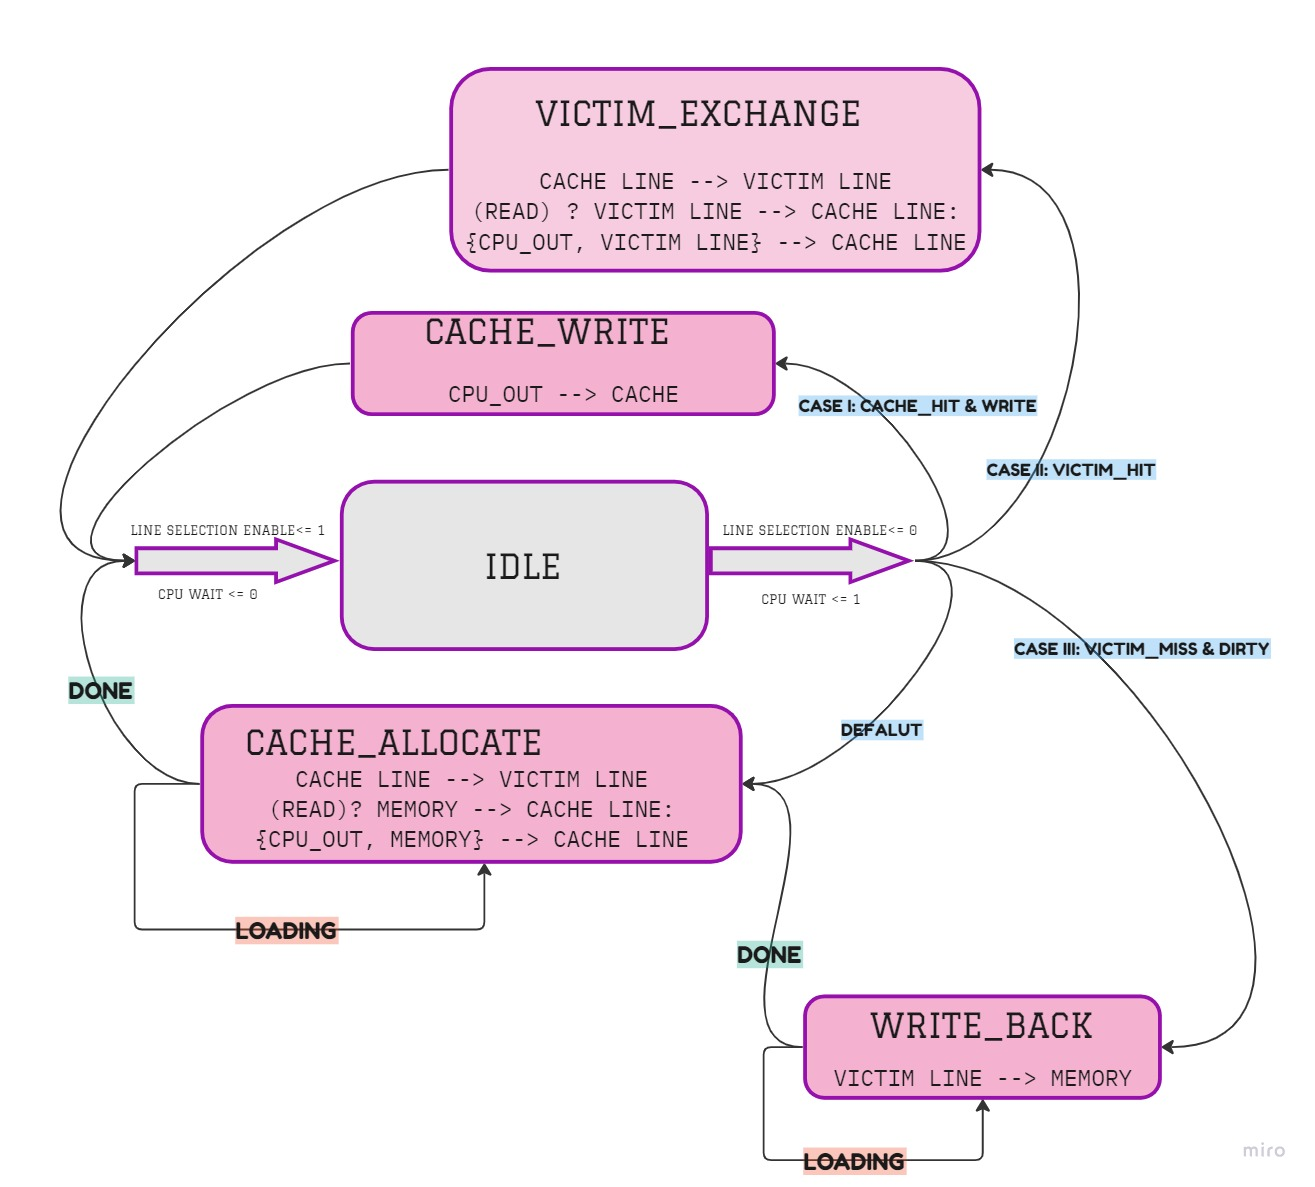
\includegraphics[width = .55\textwidth]{cache_fsm}
        \end{center}
        \caption{Cache Controller as a Finite State Machine}
    \end{figure}

    Normally the memory will be in \texttt{IDLE} state.
    When the CPU provides a valid read or write instruction,
    \begin{enumerate}
        \item The controller will check whether the data is available in the primary cache.
        Suppose the data is available and the instruction is of load type the controller will do nothing while allowing the CPU to access the data.
        \item Suppose the data is available and the instruction is of write type, the controller will turn into \texttt{CACHE\_WRITE} state and allow the CPU to write into the cache while tracking the modification via a dirty flag unique to the line.
        \item When there is a cache miss, the controller will search for the data inside the victim.
        Availability of the data into victim excites the cache into \texttt{VICTIM\_SWAP} state while allowing the data swap between the primary cache and victim cache.
        The controller is then forwarded to \texttt{IDLE} state.
        \item Victim misses together with a cache miss, trigger the controller into either one of \texttt{WRITE\_BACK} state or \texttt{CACHE\_ALLOCATE} state based on whether the selected victim line is dirty.
        Where the victim line selection will happen according to an algorithm that always preserves the most recently used three lines.
        \item On the \texttt{WRITE\_BACK} state, the dirty victim line will be written back into the memory and the controller is forwarded to \texttt{CACHE\_ALLOCATE} state.
        In this state, the data will be fetched from both memory and the CPU to put into the appropriate cache line according to the instruction.
    \end{enumerate}

    \subsection{Architecture}
    \begin{figure}[h]
        \label{fig:cache_architect}
        \begin{center}
            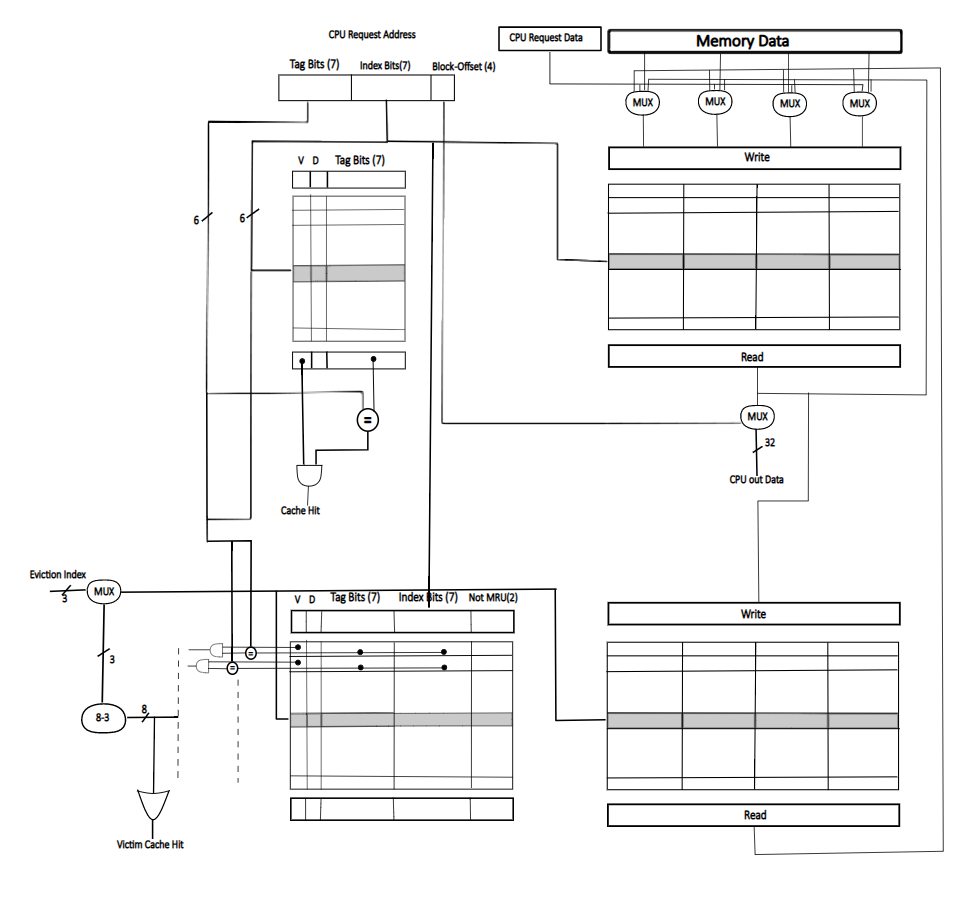
\includegraphics[width = .7\textwidth]{architect}
        \end{center}
        \caption{Memory Architecture}
    \end{figure}
    \vfill
    \\\hrule
    \href{https://gist.github.com/sanjith1999/ccd039bb128a965e286ad0d640aa9a56}{Look at the cache\_memory.v file for implementation details.}
\section{Verification of the Design}
    \subsection{Pre-stage Verifications}
    At earlier stages, simple modules are designed and verified using Modelsim integrated environment available in Quartus Prime.
    Later the core design is completely designed and simulated using \href{https://gist.github.com/dakshinatharindu}{chisel scripts}.
    After complete verification of the core processor data paths, the working of each instruction is verified using the verilator script.
    Here in the fig\ref{fig:srli} the implementation of SRLI instruction is illustrated.
    \begin{figure}[h]
        \centering
        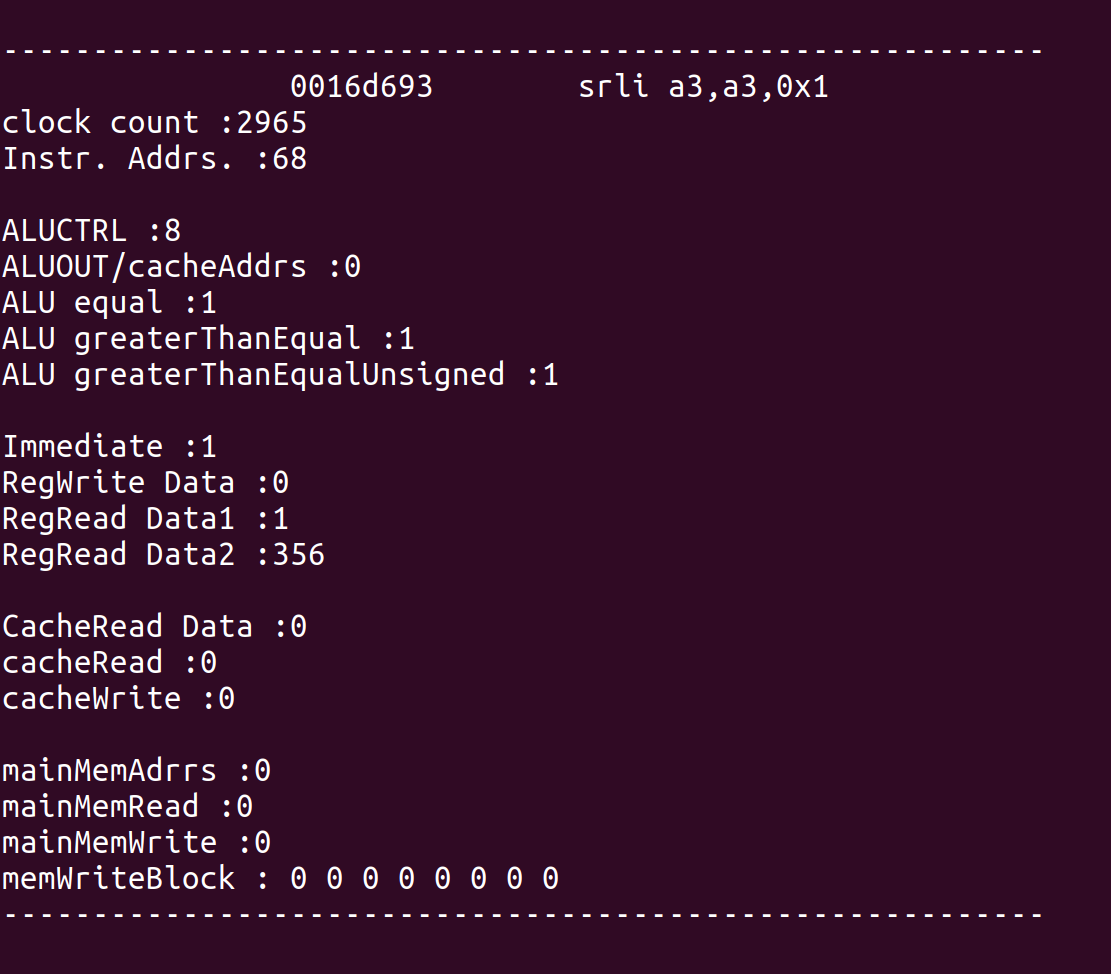
\includegraphics[width = .65\textwidth]{ver_ear}
        \caption{Processor State After an SRLI Instruction}
        \label{fig:srli}
    \end{figure}
    \subsection{Core Verification}
    The proper functioning of the design is verified by running a simple c code snippet that calculates the least common multiple of two given integers.
    \lstinputlisting[style=myStyle ,label={lst:listing-cpp}, language=C++]{./Test/code.c}
    Initially, the code snippet was converted into assembly-level instructions using the open-source \href{https://github.com/riscv-collab/riscv-gnu-toolchain}{riscv-rv32i-gcc} tool-chain to compile a given C code.
    Using a custom-made python assembler for our design, we derived binaries from the converted \href{https://gist.github.com/sanjith1999/31ac024f9fa1efea10b0b24d9ba6ecc6}{assembly-level instructions}.
    These instructions are loaded into the instruction memory using the memory content editor available with Quartus Prime Software and the data memory is monitored to check whether the expected outcome is attained.
    \par
    Register monitoring are performed using a \href{https://gist.github.com/sanjith1999/b7e914d532e387d4d3fc7dbfc8ac7b69}{Verilator} script and the results are as follows,
    We used 50 and 75 as our numbers and the least common multiple 150 is observable at the appropriate location in the cache.
    \begin{figure}[h]
        \begin{subfigure}{.95\columnwidth}
            \centering
            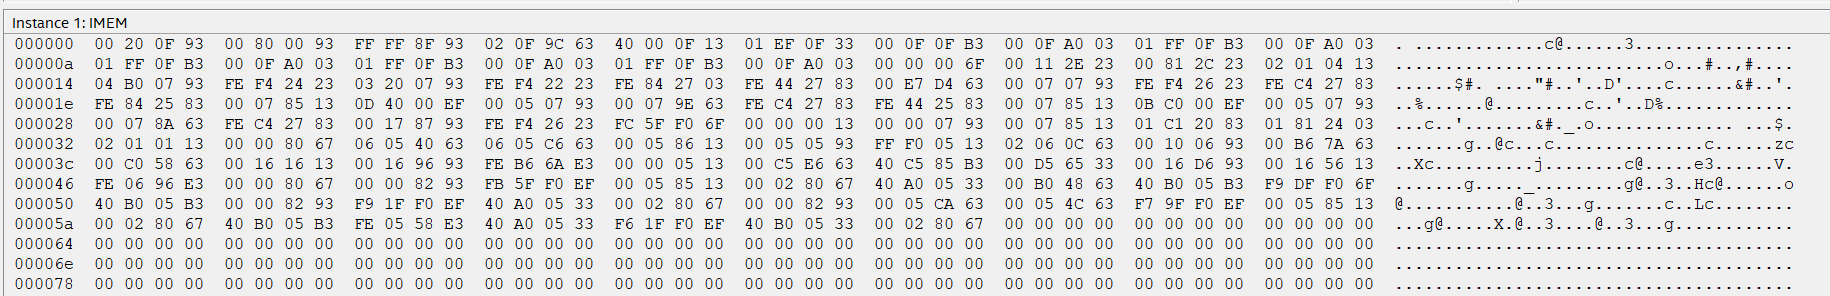
\includegraphics[width= .85\columnwidth]{im_view_qp}
            \caption{Loaded Instruction Memory}
            \label{fig:im}
        \end{subfigure}
        \begin{subfigure}{.95\columnwidth}
            \centering
            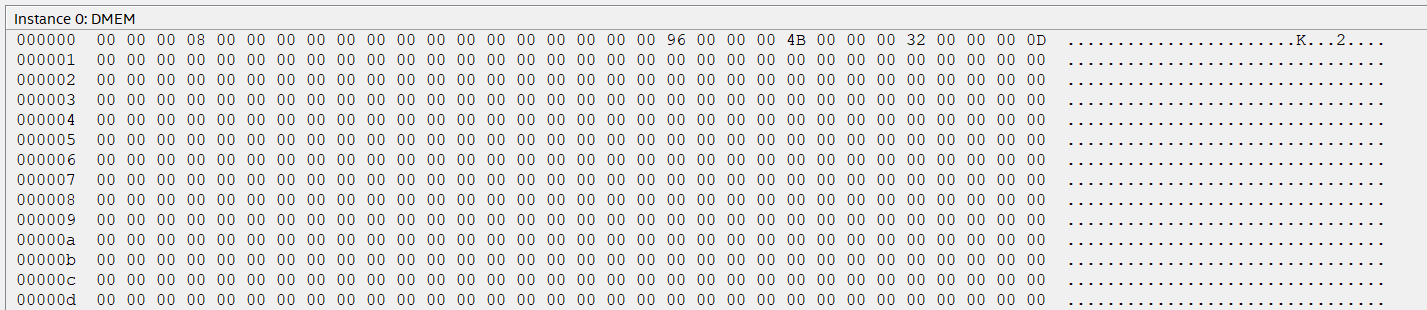
\includegraphics[width= .85\columnwidth]{dm_view_qp}
            \caption{Data Memory}
            \label{fig:dm}
        \end{subfigure}
        \begin{subfigure}{.98\columnwidth}
            \centering
            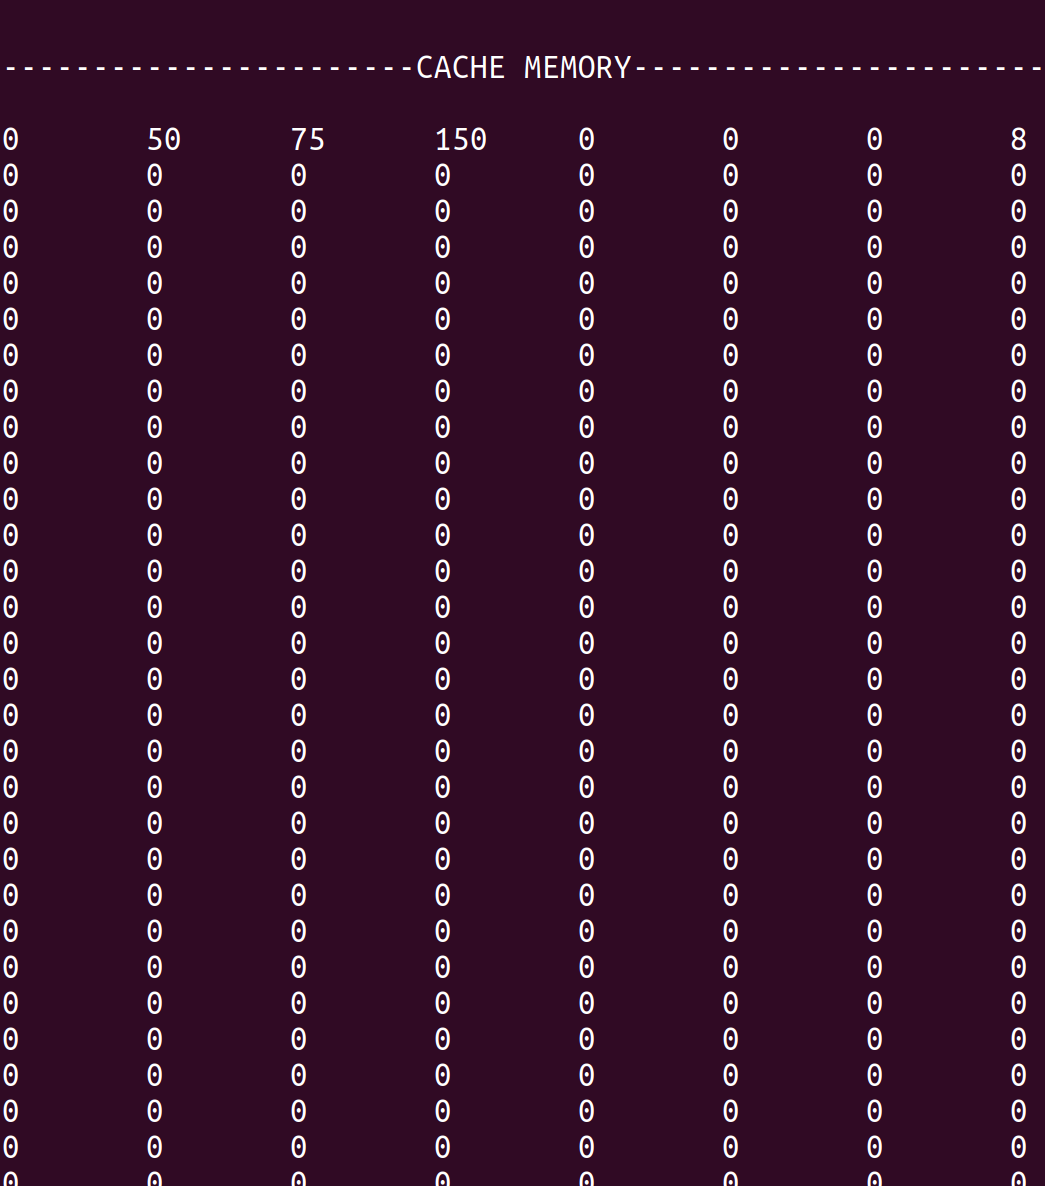
\includegraphics[width= .65\columnwidth,draft=false]{ver_lcm}
            \caption{Primary Cache Memory}
            \label{fig:ver}
        \end{subfigure}
        \caption{Monitoring the Memory Contents}
    \end{figure}
    \vfill
    \subsection{Memory Hierarchy Verification}
    Cache functions are verified completely using a \href{https://gist.github.com/sanjith1999/9955981cf15bb6e9fadb3172c60c5f10}{verilator} script and the result are as follows.
    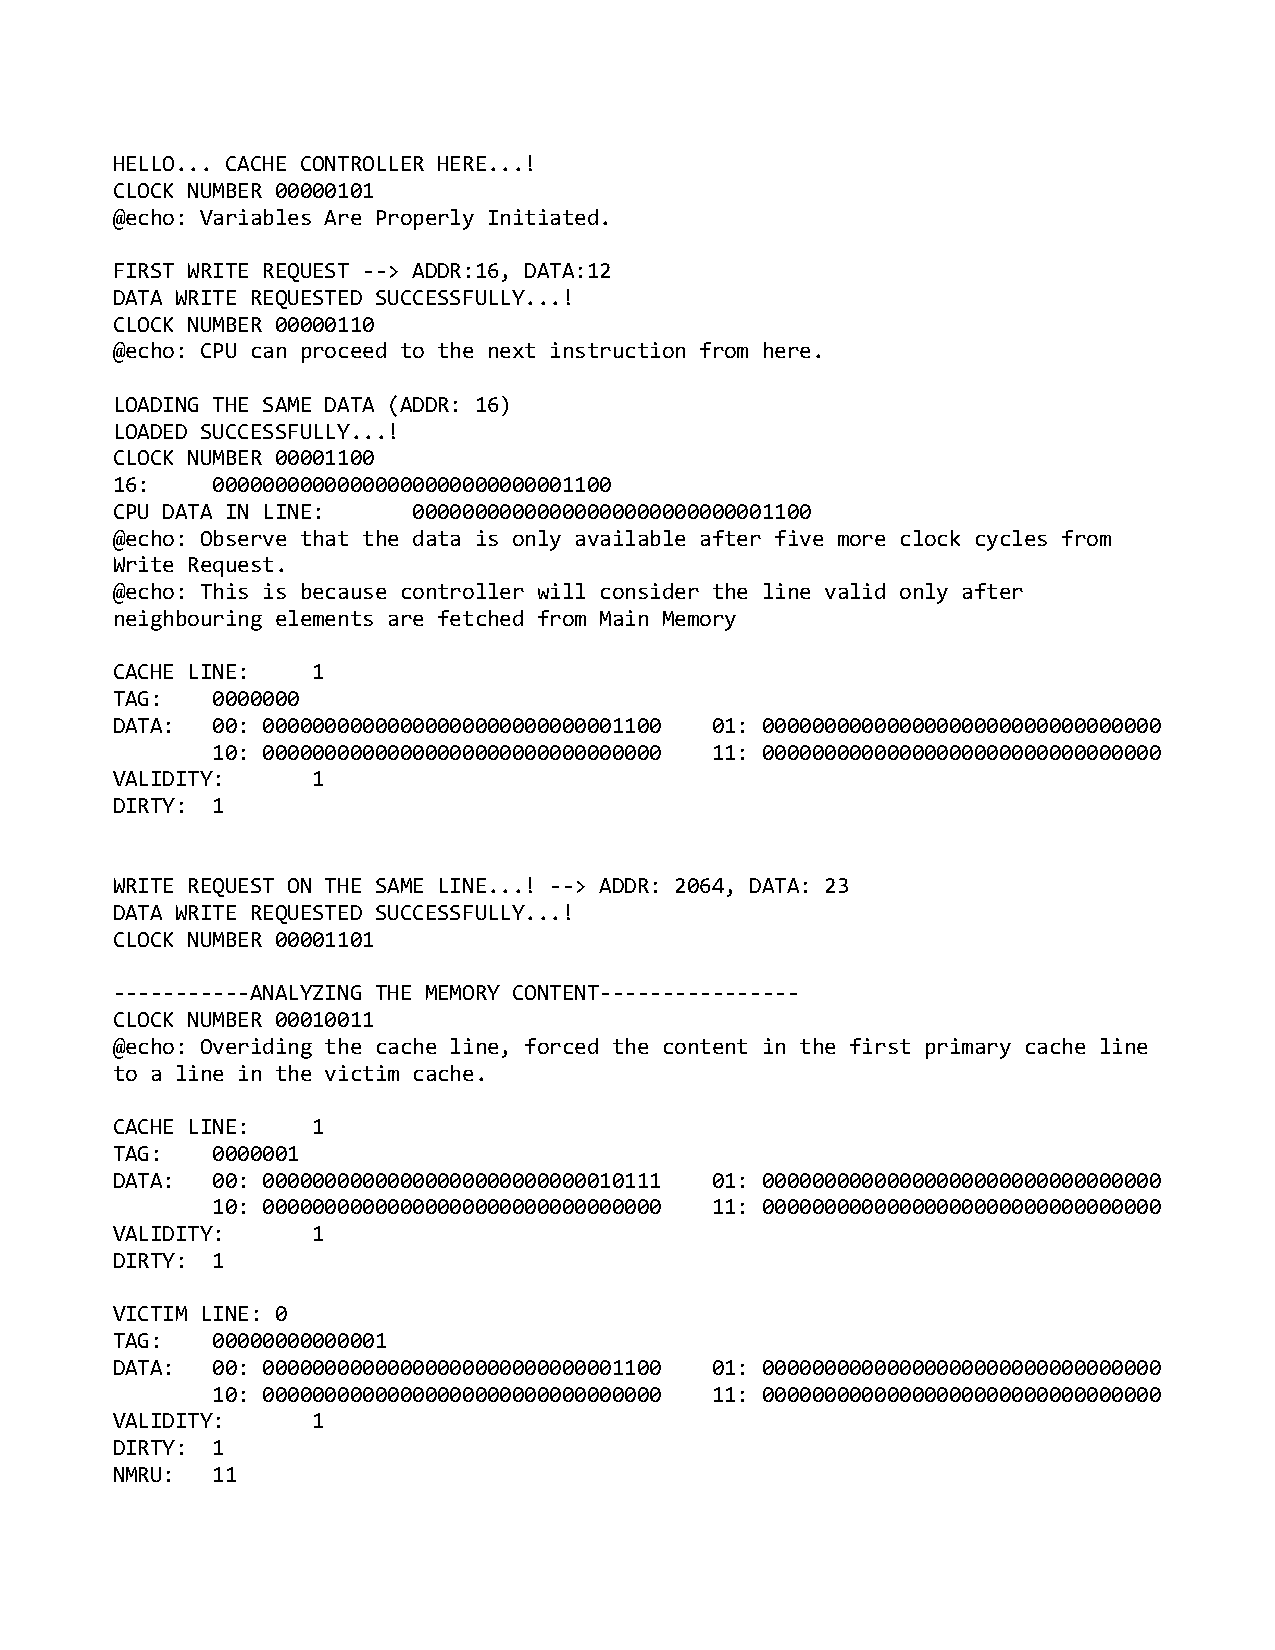
\includepdf[pages={1-5}]{./Images/cache.pdf}
    \newpage
    \appendix
    \section{Contributions}
    \begin{tabular}{|m{15em}|m{25em}|}
        \toprule
        PERSON & CONTRIBUTION\\
        \toprule\midrule
        Tharindu O.K.D - 190622R & Design and Implementation of Control Unit in Chesel. Data Path Design for CPU. Verilator Simulation of the CPU. FPGA board Implementation\\\midrule
        Sanjith. S - 190562G & Design and Implementation of Memory Hierarchy in verilog. Verification of Cache Controller with Verilator.\\\midrule
        Kajhanan. K - 190286M & Design of Memory Unit. Verilog Implementation of Eviction Unit.\\\midrule
        Yasarathna D.D.K.B. - 190719V & Verilog Implementation of ALU and Compiler Design\\\midrule
        Wansooriya W.H.O. - 190664V & Compiler Design\\\midrule
    \end{tabular}
    \vfill
    \section*{References}
    \begin{enumerate}
        \item Computer Organization and Design: the Hardware/Software Interface: Third Edition.
        \item \href{https://five-embeddev.com/riscv-isa-manual/latest/rv32.html}{Instruction Set}
        \item \href{https://github.com/paulsonkantony/risk-five}{A verilog based implemetation}
        \item \href{https://www.educative.io/answers/what-is-risc-architecture}{What is RISC architecture?}
        \item \href{https://www.youtube.com/watch?v=VNy-J0u7-jY}{RISC-V RV32I Instruction Encoding}
        \item \href{https://github.com/omega-rg/Cache-Controller}{Two-level Cache controller implementation}
    \end{enumerate}

\end{document}

\end{document}
